\chapter{Two Timing}

This is the simplest multiple-scale analysis. We can have three or even four timing etc. The two time-scales are
\begin{flalign*}
	t = \text{fast time} \\
	\tau = \epsilon t = \text{slow time}
\end{flalign*}
Regard $t$ and $\tau$ as \underline{independent} variables\footnote{One intuition behind this is that at the faster time scale, the slowly varying dynamics are practically invariant.} and write
\begin{gather*}
y(t,\epsilon) = Y(t,\tau) = Y_0(t,\tau) + \epsilon Y_1 (t,\tau) + \dots
\end{gather*}
Observing that
\begin{align*}
	\frac{\md }{\md t}y(t) = \frac{\pd }{\pd t}y(t) = \frac{\pd}{\pd t} Y(t,\tau) 
	=\frac{\pd Y}{\pd t} \cancelto{1}{\frac{\pd t}{\pd t}} + \frac{\pd Y}{\pd \tau} \cancelto{\epsilon}{\frac{\pd \tau}{\pd t}}
\end{align*}
we note for posterity
\begin{align}\label{eqn:wk23-tt-derivs}
	\begin{split}
	\dot y &= Y_t + \epsilon Y_\tau \\
	\ddot{y} &= (Y_t + \epsilon Y_\tau)_t + \epsilon (Y_t + \epsilon Y_\tau)_\tau \\
	&= Y_{tt} + 2\epsilon Y_{t\tau} + \epsilon^2 Y_{\tau \tau }
	\end{split}
\end{align}

\paragraph{Example 1:} Weakly damped linear oscillator
\begin{equation}\label{eqn:wk23-ex1-ode}
\begin{gathered}
\ddot{y} + y + 2 \epsilon \dot{y} = 0 \\
y(0) = a \qquad \dot{y}(0) = 0
\end{gathered}	
\end{equation}
Our ODE is transformed to (ignoring $O(\epsilon^2)$ terms)
\begin{align*}
	[Y_{tt} + 2\epsilon Y_{t\tau} + \cancel{\epsilon^2 Y_{\tau \tau }}] + Y + 2\epsilon[Y_t + \cancel{\epsilon Y_\tau} ] = 0
\end{align*}
Further letting
\begin{gather*}
	Y = Y_0 + \epsilon Y_1 + O(\epsilon^2)
\end{gather*}
we see that
\begin{align*}
	(Y_0 + \epsilon Y_1)_{tt} + 2\epsilon (Y_0)_{t\tau} + (Y_0 + \epsilon Y_1) + 2\epsilon (Y_0)_{t} = 0
\end{align*}
Solving the $O(1)$ problem
\begin{gather*}
	(Y_0)_{tt} + Y_0 = 0 \qquad 
\end{gather*}
yields\footnote{Expanding the expression below it is easy to see that this is the most general \emph{real} solution: $Y_0 = 2A_r \cos t - 2A_i \sin t$. This form is advantageous as we would only need to do half as much writing.}
\begin{align*}
	Y_0 &= A \me^{\mi t} + \underbrace{A^\ast \me^{-\mi t}}_\text{c.c}
\end{align*}
where $A=A_r + \mi A_i$ is a complex number and $A^\ast$ its complex conjugate. Since $Y_0 = Y_0(t,\tau)$, it must be that the ``constant'' $A=A(\tau)$. This further provides the intuition that the amplitude is changing on the slow time scale $\tau$. The $O(\epsilon)$ ODE is
\begin{align*}
	(Y_1)_{tt} + Y_1 &= -2(Y_0)_t - 2(Y_0)_{t\tau} \\
	&= -2\mi (A + A_\tau) \me^{\mi t} + \text{c.c.}
\end{align*}
Note that we have a resonant forcing term on the right hand side, which would lead to a secular growth unless this is forced to zero. This provides us with an ``amplitude equation''
\begin{gather*}
	A_\tau + A = 0 \quad \implies A(\tau) = A(0)\me^{-\tau}
\end{gather*}
Satisfying this removes the secularity at this order in $\epsilon$. The next task is to work out the ICs:
\begin{align*}
	y(0) = Y(0,0) = Y_0(0,0) + \epsilon Y_1(0,0) + \dots &= a \qquad \forall \epsilon \\
	Y_0(0,0) &= a \\ 
	Y_1(0,0) &= 0 \\
	\vdots \\
	\dot y(0) = Y_t+ \epsilon Y_\tau = (Y_0)_t + \epsilon [(Y_1)_t + (Y_0)_\tau] + \dots &= 0 \qquad \forall \epsilon\\
	(Y_0)_t(0,0) &= 0 \\
	(Y_1)_t(0,0) + (Y_0)_\tau(0,0) &= 0 \\
	\vdots 
\end{align*}
We next use these ICs on our $O(1)$ solution
\begin{gather*}
	Y_0 = A(0)\me^{-\tau} \me^{\mi t} + \text{c.c.} \\
	Y_0(0,0) = A(0) + A^\ast(0) = 2 \text{Re}[A(0)] = a \\
	(Y_0)_t(0,0) = -2 \text{Im}[A(0)] = 0
\end{gather*}
Altogether
\begin{align}
	Y_0 &= \frac{a}{2} \me^{-\epsilon t} \me^{\mi t} + \text{c.c.} + O(\epsilon) \nonumber \\
	&=a \me^{-\epsilon t} \cos t + O(\epsilon) \label{eqn:wk23-ex1-anasol}
\end{align}
This result is asymptotically valid for $\epsilon \rightarrow 0^+$, uptil $\tau = \epsilon t = O(1)$. Comparison of the analytical and numerical solutions are shown in Fig. \ref{fig:wk23-ex1}.\\
\ \newline
It is worth noting that in calculating $Y_1$, the secular term was eliminated. The solution will remain bounded at $O(\epsilon)$. The secularity is in fact pushed to the $O(\epsilon^2)$ term and appears at a $\epsilon^2 t$ time scale. To push the secular term even further out in time, we would need to perform a three time scale analysis!
\begin{figure}[!h]
	\centering
	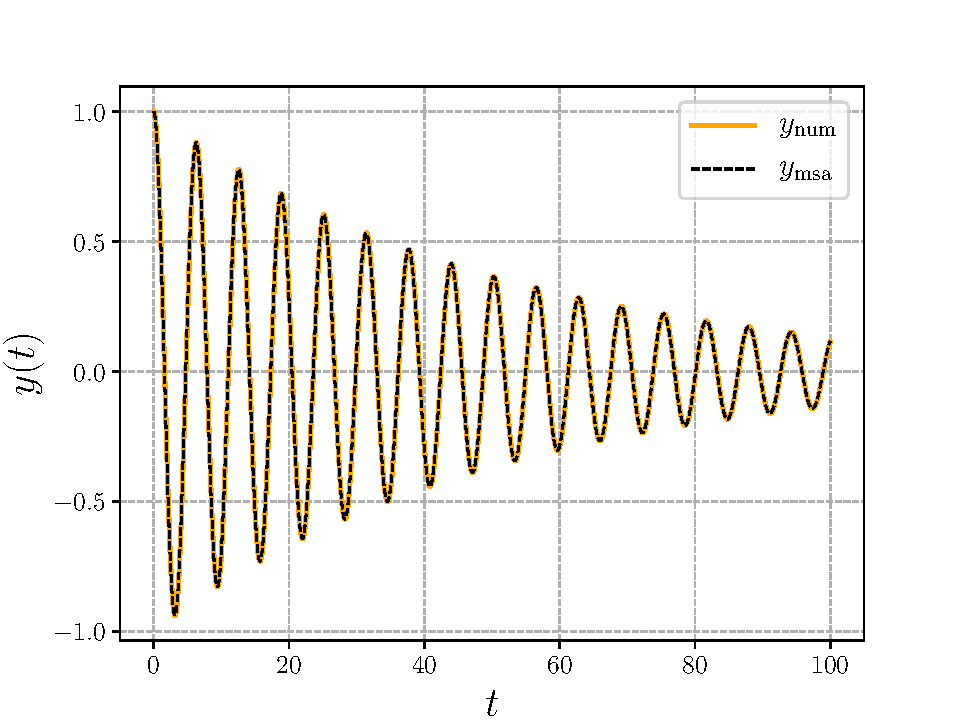
\includegraphics[width=0.7\textwidth]{./plots/pdf/strogatz-wk23-ex1.pdf}
	\caption{Plots of direct numerical solution to eqn. \ref{eqn:wk23-ex1-ode} and its analytical solution eqn. \ref{eqn:wk23-ex1-anasol} for $\epsilon=0.02$ and $a=1$.}
	\label{fig:wk23-ex1}
\end{figure}\\

\paragraph{Example 2:} The van der Pol oscillator
\begin{gather}
	\ddot{y} + \epsilon \dot{y}(y^2 -1) + y = 0, \qquad 0 < \epsilon \ll 1 \label{eqn:wk23-ode-vdP}
\end{gather}
Observe that if $|y|>1$, the nonlinear $\epsilon$ term acts like an ordinary damping. However as the amplitude falls to $|y|<1$, energy is pumped into the oscillator. We therefore expect the system to settle into some ``limit cycle'', which is a self-sustained oscillation whose amplitude is independent of the ICs. We will answer a couple of questions:
\begin{enumerate}
	\item How do solutions approach the limit cycle?
	\item For $\epsilon=0$, \underline{any} amplitude solution is admissible. However for $0<\epsilon \ll 1$, an approximate amplitude of the limit cycle can be determined.
\end{enumerate}
Proceeding as previously, recall
\begin{align*}
	\dot y &= Y_t + \epsilon Y_\tau \\
	\ddot{y} &= Y_{tt} + 2\epsilon Y_{t\tau} + \epsilon^2 Y_{\tau \tau }
\end{align*}
which transforms the vdP equation to
\begin{gather*}
	(Y_{tt} + 2\epsilon Y_{t\tau} + \dots ) + \epsilon ( Y_t + \dots) (Y^2-1) + Y = 0 \\
	(Y_0 + \epsilon Y_1)_{tt} + 2 \epsilon (Y_0)_{t\tau} + \epsilon (Y_0)_t (Y_0^2-1) + (Y_0 + \epsilon Y_1) + O(\epsilon^2) = 0
\end{gather*}
Collecting terms
\begin{align*}
	O(\epsilon^0): \qquad & \ddot Y_0 + Y_0 = 0\\
	O(\epsilon^1): \qquad & \ddot Y_1 + Y_1 = -2 (Y_0)_{t\tau } - (Y_0^2-1)(Y_0)_t
\end{align*}
The $O(1)$ solution is
\begin{gather*}
	Y_0(t,\tau) = A(\tau) \me^{\mi t} + A^\ast (\tau) \me^{-\mi t} 
\end{gather*}
The $O(\epsilon)$ equation is
\begin{align*}
	\ddot Y_1 + Y_1 = &-2(\mi A_\tau \me^{\mi t} + \text{c.c.}) \\
	&- (A^2 \me^{2\mi t} + (A^\ast)^2 \me^{-2\mi t} + 2 |A|^2-1)(\mi A \me^{\mi t} -\mi A^\ast \me^{-\mi t}) \\
	=& \me^{\mi t} \left[ -2 \mi A_\tau + \mi A^2 A^\ast - \mi A(2 |A|^2-1) \right] + \me^{3\mi t}[-\mi A^3] + \text{c.c.}
\end{align*}
The resonant forcing is the term which multiplies the $\me^{\mi t}$ term. This will produce secular terms in $Y_1$ unless we force this to zero.
\begin{gather}
	2 A_\tau + A |A|^2 - A = 0 \label{eqn:wk23-ex2-ode-amp}
\end{gather}
The solution of the \emph{complex} amplitude equation is found by proceeding with the ansatz
\begin{gather}
	A(\tau) = R(\tau) \me^{\mi \theta(\tau )} \label{eqn:wk23-evelope-ansatz}
\end{gather}
We think the problem will have a circular limit cycle (weakly deviating from the simple harmonic motion), so the polar coordinate ansatz is a natural move. With this eqn. \ref{eqn:wk23-ex2-ode-amp} reads
\begin{gather*}
	2 (R' + \mi R \theta') \me^{\mi \theta} = (R - R^3)\me^{\mi \theta}
\end{gather*}
Equating the real and imaginary parts:
\begin{align*}
	R' &= \frac{1}{2} R(1-R^2) \\
	\theta ' &= 0
\end{align*}
At this order of perturbation theory, there is no phase drift (unlike the Duffing oscillator), i.e. $\theta = \theta_0$ (constant). The system in $R$ is a Bernoulli differential equation and can be solved with the substitution  
\begin{gather*}
	u = \frac{1}{R^2}
\end{gather*}
This yields
\begin{gather*}
	u' = 1 - u
\end{gather*}
Solving with the integrating factor
\begin{gather*}
	u(\tau) = 1 + C\me^{-\tau}
\end{gather*}
With the initial condition $R(0)= R_0$, we derive $C = R_0^{-2}-1$ to write
\begin{gather*}
	R(\tau ) = [1+(R_0^{-2}-1)\me^{-\tau}]^{-1/2}
\end{gather*}
Pulling everything together
\begin{align}
	Y_0 &= A(\tau) \me^{\mi t} + \text{c.c} \nonumber \\
	&= R(\tau) \me^{\mi (\theta_0 + t)}+ \text{c.c} \nonumber \\
	&= 2 R(\tau) \cos (t+\theta_0) \nonumber \\
	y(t,\epsilon) &\sim \frac{2 \cos (t+\theta_0)}{\sqrt{1+(R_0^{-2}-1)\me^{-\epsilon t}}} + O(\epsilon) \label{eqn:wk23-vdP-ana}
\end{align}
Therefore as $t \rightarrow \infty$, $y \rightarrow 2 \cos (t+\theta_0)$, i.e. the amplitude goes to 2.
\begin{figure}[!h]
	\centering
	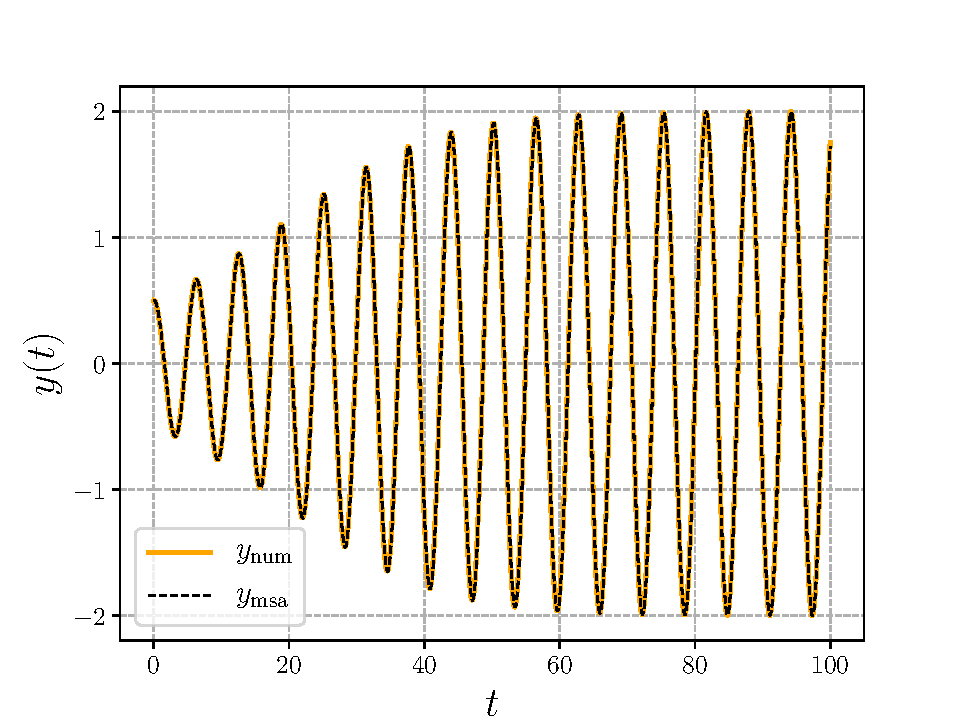
\includegraphics[width=0.7\textwidth]{./plots/pdf/strogatz-wk23-vdP.pdf}
	\caption{Plots of direct numerical solution to eqn. \ref{eqn:wk23-ode-vdP} and its analytical solution eqn. \ref{eqn:wk23-vdP-ana} for $\epsilon=0.1$ and $y(0)=1/2$ and $\dot{y}(0)=0$.}
	\label{fig:wk23-ex2-vdP}
\end{figure}\\

\paragraph{Example 3:} Duffing (eqn. \ref{eqn:duffing}) revisited...
\begin{gather*}
\ddot{y} + y + \epsilon y^3 = 0, \qquad 0 < \epsilon \ll 1 \\
y(0) = 1 \qquad \dot y(0) = 0 \nonumber 
\end{gather*}
Using eqns. \ref{eqn:wk23-tt-derivs} our ODE becomes
\begin{gather*}
(Y_{tt} + 2\epsilon Y_{t\tau} + \dots ) + y + \epsilon y^3 = 0 \\
(Y_0 + \epsilon Y_1 )_{tt} + 2\epsilon (Y_0)_{t\tau} + (Y_0 + \epsilon Y_1) + \epsilon Y_0^3 + O(\epsilon^2) = 0
\end{gather*}
Equating powers of $\epsilon$:
\begin{align*}
(Y_0)_{tt} + Y_0 &= 0 \\
(Y_1)_{tt} + Y_1 &= -Y_0^3 -2 (Y_0)_{t\tau}
\end{align*}
The general solution to the $O(1)$ eqn. is
\begin{gather*}
Y_0 = A(\tau) \me^{\mi t} + A^\ast (\tau) \me^{-\mi t}
\end{gather*}
which upon substitution into the $O(\epsilon)$ yields
\begin{align*}
(Y_1)_{tt} + Y_1 =& -A^3 \me^{3\mi t} - A^{\ast 3}\me^{-3\mi t} \\
&+ \left( -3A^2 A^\ast - 2\mi A_\tau \right) \me^{\mi t} + \left(-3 A A^{\ast 2} + 2\mi  A^\ast_ \tau \right) \me^{-\mi t}
\end{align*}
To ensure that there are no secular terms in $Y_1$, the resonant terms on the right hand side are forced to zero, i.e.
\begin{gather*}
2 \mi A_\tau + 3 |A|^2 A = 0 
\end{gather*}
Substitute eqn. \ref{eqn:wk23-evelope-ansatz} into the above equation:
\begin{gather*}
-2 R \theta_\tau + 2 \mi R_\tau + 3 R^3 = 0
\end{gather*}
Upon equating the real and imaginary parts to zero and integrating
\begin{gather*}
R(\tau) = R_0 \\
\theta(\tau) = \theta_0 + \frac{3}{2} R^2_0  \tau
\end{gather*}
Collecting everything
\begin{gather*}
Y_0 = 2 R_0 \cos \left(t + \theta_0 + \frac{3}{2} R_0^2 \epsilon t\right)
\end{gather*}
Applying the initial conditions we derive
\begin{gather*}
1 = 2 R_0 \cos \theta_0 \\
0 = -2 R_0 \left(1 + 3R_0^2 \epsilon/2\right)\sin \theta_0 
\end{gather*}
Therefore $R_0 = 1/2$ and $\theta_0 = 0$, yielding
\begin{gather}\label{eqn:duffing-analytic}
y(t) = \cos \left(t + 3\epsilon t / 8\right) + \mathcal{O}(\epsilon)
\end{gather}
Higher order terms in the expansion are generated by systematically eliminating secular terms at each order. The \emph{method of averaging} can also be used to derive this result (sec. \ref{sec:moa-duffing}). 

